\subsection{Aloo Gobi (curry de papas con coliflor)}
\underline{Ingredientes}
\begin{itemize}
\item 1 coliflor
\item 3 papas medianas
\item 2 cebollas moradas
\item Aceite de canola para freir
\item 2 jitomates
\item Muchas especias m\'agicas
\item $1 \frac{1}{2} - 2$ cucharadas de pasta de ajo y gengibre
\item $1/2 - 1$ cucharaditas de tumeric
\item $1 - 1 \frac{1}{2}$ cucharaditas de chile rojo en polvo
\item $2 - 2 \frac{1}{2}$ cucharaditas de comino con cilantro (cumin-coriander)
\item 1 pizca de garam masala ($< 1/2$ cucharadita)
\item cilantro para decorar

\end{itemize}

\underline{Instrucciones}

\begin{enumerate}
\item Cortar la coliflor en floretes medianos.
\item Freir la coliflor en aceite primero a fuego medio-alto para que se dore. Una vez que est\'e dorada reducir el fuego y tapar para que se suavice un poco. Tener cuidado de que no se suavice demasiado porque se puede cocer demaciado y desbaratarse al final. 
\item Partir las cebollas moradas en cuatro pedazos y luego cortar en tiras no muy delgadas (ver figura)
\item Mientras se cocinan las cebollas partir las papas en cubos medianos. 
\item Una vez que est\'en cocidas las cebollas agragar las papas y cubrir. Dejar cocer las papas con la cebolla a fuego medio hasta que se suavicen, moviendo cada dos o tres minutos para que no se peguen. Las papas est\'an listas cuando se pueden cortar con una esp\'atula sin hacer mucha fuerza (no tienen que estar completamente cocidas ahora, solo un poco suaves).
\item Ankit recomienda que al final queden cebollas a diferente nivel de dorado, unas cafecitas y otras no tanto, para añadirle complejidad.
\item Cuando est\'en listas las papas reducir el fuego a medio bajo y agregar la pasta de ajo con gengibre. Hay que tener cuidado porque tiende a pegarse al fondo del sart\'en y amarga el sabor. Es importante revolverlo bien para que no se queme. Ankit dice que est\'a listo cuando tiene un aroma dulce pero el olor a ajo ya no es tan intenso.
\item Agregar las especias: primero tumeric y chile. Las papas deben verse de un color amarillento-naranja como en la foto. 
\item Agregar la mezcla de comino con cilantro (esta mezcla se vende en las tiendas indues pero se puede hacer en casa mezclando los dos ingredientes a partes iguales). Ankit dice que en general se le puede agregar mucho de este condimento a los platillos porque da mucho sabor pero tampoco enmascara los otros sabores. 
\item Agregar el garam masala. Cuidado porque este condimento es muy fuerte! 
\item Agregar la coliflor a las papas y revolver con cuidado para que no se rompan. 
\item Este es el ultimo momento en el que se pueden ajustar las especias (excepto el chile, de ese si se puede agregar m\'as despu\'es). Probar una papa y ajustar especias al gusto. 
\item Cortar los jitomates en pedazos medianos-grandes. Hacer un pozo en medio de la cacerola y poner ah\'{\i} los jitomates. Ankit recomienda que no se agreguen especias como el garam masala o el comino-cilantro despu\'es de agregar los jitomates a la mezcla porque tienden a soltar l\'{\i}quido y las especias no se `cuecen' bien. 
\item Cubrir la cacerola y dejar cocer a fuego lento. De vez en cuando se puede abrir para aplastar los jitomates
\item Cuando esten suaves los jitomates mezclar todo y agragar un poco de agua al gusto. Si se va a comer con arroz agregar m\'as agua para que quede una salsa 

\begin{figure}[H]
\centering
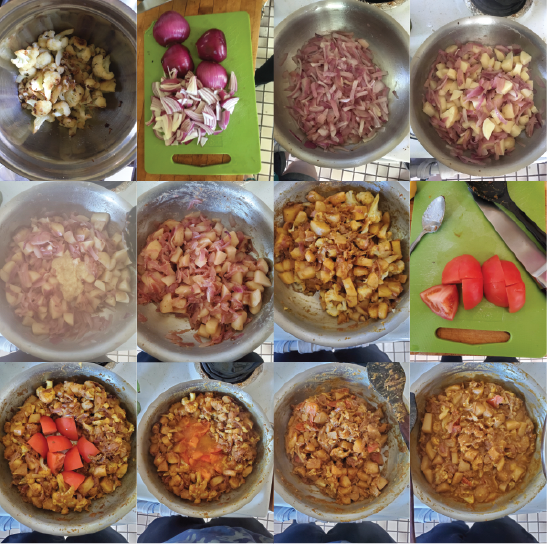
\includegraphics[width=1\textwidth]{recetas/Aloo-gobi/aloo-gobi.png}
\caption{Progresi\'on de la receta}
\label{fig:aloo-gobi}
\end{figure}

\end{enumerate}